\documentclass[14pt,fleqn]{extarticle}
\RequirePackage{prepwell}
\previewoff
\begin{document}

\newcommand\inta{\int_{-6}^{-3}}
\newcommand\intb{\int_{-3}^0}
\newcommand\fx{\left(\frac{x^2}{2} + 3x\right)}

%text
Sketch the graph of $y=\vert x + 3\vert$ and evaluate
the area under the curve $y=\vert x+3\vert$, above 
the $x-$axis and between $x=-6$ to $x=0$.
%

\newcard

Just as 
\small$ f(x) = \vert x\vert = \begin{cases} 
x,\quad x\geq 0 \\
-x,\quad x < 0 
\end{cases} $\normalsize \newline 

Similarly 

\small$y = \vert x+3\vert = \begin{cases}
x+3,\, x+3 \geq 0 \implies x \geq -3 \\
-\left(x+3 \right),\, x+3 < 0 \implies x < -3 
\end{cases}$ \normalsize\newline 

Which is why the graph of $y=\vert x+3\vert$ looks like the one below 

\begin{center}
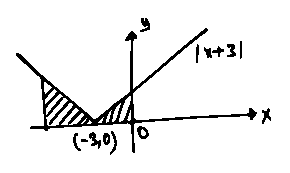
\includegraphics[scale=1.6]{modx.eps} 
\end{center} 

The required area is the shaded bit 

\newcard 

The required area $R$ is therefore 

\[ R = -\inta \left(x+3 \right)\cdot dx + \intb \left(x+3 \right)\cdot dx \]

\newcard 

From $x=-6\rightarrow -3$, we need the area under $y = - \left(x+3 \right)$\newline 

And from $x=-3\rightarrow 0$, we need the area under $y = \left(x+3 \right)$\newline 

And hence 
\[ R = -\inta \left(x+3 \right)\cdot dx + \intb \left(x+3 \right)\cdot dx \]

\newcard 

\[ \qquad R = 9\text{ sq. units} \]

\newcard 

 \[ \qquad R = 18\text{ sq. units} \]
 
 \newcard 
 
 \begin{align}
 R &= -\inta \left(x+3 \right)\cdot dx + \intb \left(x+3 \right)\cdot dx \\
 &= - \left[\fx \right]_{-6}^{-3} + \left[\fx \right]_0^3 \\
 &= -\left[\left(\frac{9}{2}-9\right) - \left(18-18\right) \right] + \left[0-\left(\frac{9}{2}-9\right)\right]\\
 &= \frac{9}{2} - \frac{9}{2} + 9 = 9\text{ sq units}
\end{align}
\end{document}